\begin{titlepage}

  \setlength{\parindent}{0pt}
  \thispagestyle{empty}

  \begin{center}
  
\includegraphics[height=3cm]{content/logo}
  \end{center}

  \bigskip

  \begin{center}
  \fontsize{14pt}{16pt}\selectfont
  \textbf{THÈSE DE DOCTORAT DE L'UNIVERSITÉ DE LYON}\\

  \bigskip

  \fontsize{12pt}{14pt}\selectfont
  \textbf{Opérée au sein de}\\ \medskip
  l'Université Claude Bernard Lyon 1

  \textbf{École doctorale}\\ \medskip
  Neurosciences et Cognition (ED476)

  \textbf{Spécialité de doctorat}\\ \medskip
  Neurosciences

  Soutenue publiquement le 8 décembre 2017 par\\ \medskip
  \fontsize{14pt}{16pt}\selectfont
  \textbf{\thesisName}

  \rule{\textwidth}{0.5pt}

  \fontsize{16pt}{20pt}\selectfont
  FRÉQUENCE ET CONTENU DU RAPPORT DE RÊVE:\\ \medskip
  Approches Comportementales et Neurophysiologiques.
  \rule{\textwidth}{0.5pt}

  \end{center}

  \fontsize{12pt}{14pt}\selectfont
  \textbf{Devant le jury composé de:}

  Pr. Sophie Schwartz  	\hfill Rapporteure\\
  Pr. Michael Schredl 	\hfill Rapporteur\\
  Pr. Yves Rossetti 	\hfill Examinateur\\
  Dr. Perrine Ruby 		\hfill Directrice de thèse\\

  \vfill

\end{titlepage}

\cleardoublepage
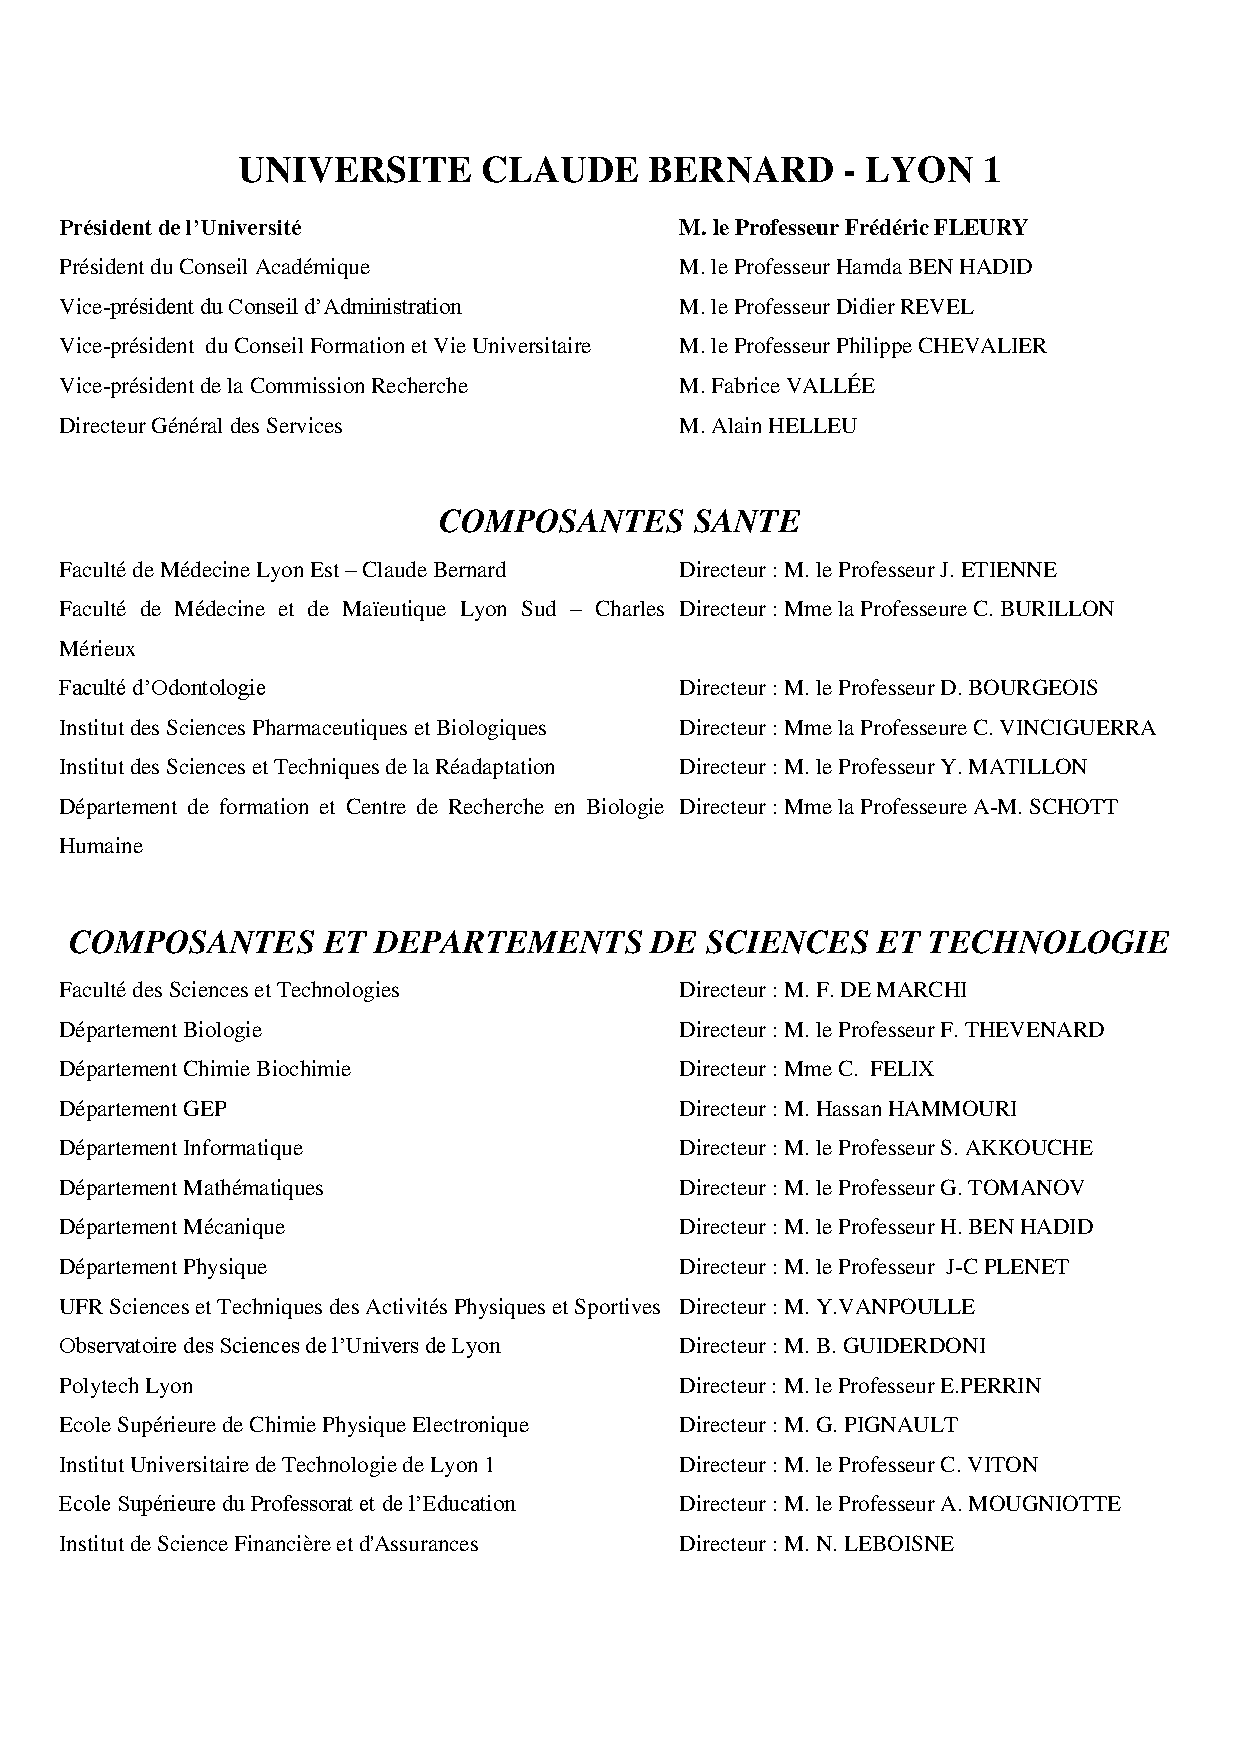
\includepdf[pages=-, fitpaper=true]{content/composante_lyon1.pdf}
